\documentclass[handout]{beamer}
\usetheme{metropolis}
\beamertemplatetransparentcoveredhigh

\usepackage[portuges]{babel}
\usepackage{graphicx}
\graphicspath{{./figs/}}
\usepackage{listings}
\usepackage{color}
\usepackage{hyperref}
\usepackage{xpatch}
\usepackage{comment}
\usepackage[outputdir=build]{minted}

\makeatletter
\AtBeginEnvironment{minted}{\dontdofcolorbox}
\def\dontdofcolorbox{\renewcommand\fcolorbox[4][]{##4}}
\xpatchcmd{\inputminted}{\minted@fvset}{\minted@fvset\dontdofcolorbox}{}{}
\xpatchcmd{\mintinline}{\minted@fvset}{\minted@fvset\dontdofcolorbox}{}{}
\makeatother
\setminted[c]{
  linenos=true,
  breaklines=true,
  encoding=utf8,
  frame=lines,
  framerule=0.5pt,
  autogobble,
  fontsize=\small,
}
\setminted[bash]{
  linenos=true,
  encoding=utf8,
  frame=lines,
  framerule=0.5pt,
  autogobble,
  fontsize=\small
}

\newcommand{\cod}[1]{\mintinline{c}{#1}}


\definecolor{dkgreen}{rgb}{0,0.6,0}
\definecolor{gray}{rgb}{0.5,0.5,0.5}
\definecolor{mauve}{rgb}{0.58,0,0.82}


\definecolor{Purple}{HTML}{911146}
\definecolor{Orange}{HTML}{CF4A30}
\setbeamercolor{alerted text}{fg=Orange}
\setbeamercolor{frametitle}{bg=Purple}
\setbeamercolor{block body}{bg=Purple!20,fg=black}
\setbeamercolor{block title}{bg=Purple!50,fg=black}
\setbeamertemplate{blocks}[rounded][shadow=true]


\newcounter{ExercicioCounter}
\newcommand{\exercicio}{\refstepcounter{ExercicioCounter} Exercício~\theExercicioCounter}

\newcommand{\setcoverbg}{
  \setbeamertemplate{background}
  {
\includegraphics[width=\paperwidth,height=\paperheight]{backgrounds/coverbg}}
}
\newcommand{\setsectionbg}{
  \setbeamertemplate{background}
  {
\includegraphics[width=\paperwidth,height=\paperheight]{backgrounds/blank}}
}

\title{Programação Estruturada}
\subtitle{Registros (\emph{structs})}

\author{Professores Emílio Francesquini e Carla Negri Lintzmayer}
\institute{Centro de Matemática, Computação e Cognição\\ Universidade
  Federal do ABC} \date{2018.Q3}

\begin{document}

\setcoverbg
\maketitle
\setsectionbg

%%%%%%%%%%%%%%%%%%%%%%%%%%%%%%%%%%%%%%%%%%%%%
%%%%%%%%%%%%%%%%%%%%%%%%%%%%%%%%%%%%%%%%%%%%%
%%%%%%%%%%%%%%%%%%%%%%%%%%%%%%%%%%%%%%%%%%%%%
%%%%%%%%%%%%%%%%%%%%%%%%%%%%%%%%%%%%%%%%%%%%%
%%%%%%%%%%%%%%%%%%%%%%%%%%%%%%%%%%%%%%%%%%%%%
%%%%%%%%%%%%%%%%%%%%%%%%%%%%%%%%%%%%%%%%%%%%%
\section{Registros}

%%%%%%%%%%%%%%%%%%%%%%%%%%%%%%%%%%%%%%%%%%%%%
\begin{frame}{Registros}

    \begin{block}{}
        Um registro é um mecanismo da linguagem C para agrupar várias
        variáveis, que inclusive podem ser de tipos diferentes, mas
        que dentro de um contexto, fazem sentido estarem juntas.
    \end{block}

    \begin{itemize}
        \item Exemplos de uso de registros:
        \begin{itemize}
            \item Registro de alunos para guardar os dados: nome, RA,
            médias de provas, médias de labs, etc\ldots
            \item Registro de pacientes para guardar os dados: nome,
            endereço, histórico de doenças, etc\ldots
        \end{itemize}
    \end{itemize}

\end{frame}

%%%%%%%%%%%%%%%%%%%%%%%%%%%%%%%%%%%%%%%%%%%%%
%%%%%%%%%%%%%%%%%%%%%%%%%%%%%%%%%%%%%%%%%%%%%
%%%%%%%%%%%%%%%%%%%%%%%%%%%%%%%%%%%%%%%%%%%%%
\subsection{Declarando um novo tipo de registro}

%%%%%%%%%%%%%%%%%%%%%%%%%%%%%%%%%%%%%%%%%%%%%
\begin{frame}[fragile]{Declarando um novo tipo de registro}

    \begin{itemize}
        \item Para criarmos um novo tipo de registro usamos
        a palavra chave \textbf{struct} da seguinte forma:

        \begin{minted}{c}
            struct nome_registro {
                tipo_1 nome_campo_1;
                tipo_2 nome_campo_2;
                tipo_3 nome_campo_3;
                ...
                tipo_n nome_campo_n;
            };
        \end{minted}

        \item Cada \textbf{nome\_campo\_i}, é um identificador que
        será do tipo \textbf{tipo\_i} (são declarações de variáveis
        simples).
    \end{itemize}
\end{frame}

%%%%%%%%%%%%%%%%%%%%%%%%%%%%%%%%%%%%%%%%%%%%%
\begin{frame}[fragile]{Declarando um novo tipo de registro}

    Exemplo:
    \begin{minted}{c}
        struct Aluno {
            char nome[80];
            float nota;
        };  /* estamos criando um novo tipo "struct Aluno" */
    \end{minted}

\end{frame}


%%%%%%%%%%%%%%%%%%%%%%%%%%%%%%%%%%%%%%%%%%%%%
\begin{frame}[fragile]{Declarando um novo tipo de registro}

    A declaração do registro pode ser feita dentro
    de uma função ou fora dela. Usualmente, ela
    é feita fora de qualquer função, para que qualquer função
    possa usar dados do tipo de registro criado.

    \begin{minted}{c}
        #include <stdio.h>

        /* Declare tipos registro aqui */

        int main() {
            /* Comandos */
        }
    \end{minted}

\end{frame}

%%%%%%%%%%%%%%%%%%%%%%%%%%%%%%%%%%%%%%%%%%%%%
\begin{frame}[fragile]{Declarando um registro}

    A próxima etapa é declarar uma variável do tipo
    \textbf{struct nome\_registro}, que
    será usada dentro de seu programa, como no exemplo abaixo:

        \begin{minted}{c}
            #include <stdio.h>

            struct Aluno {
                char nome[80];
                float nota;
            };

            int main() {
                /* variáveis são do tipo "struct Aluno" */
                struct Aluno a, b;
                ...
            }
        \end{minted}

\end{frame}

%%%%%%%%%%%%%%%%%%%%%%%%%%%%%%%%%%%%%%%%%%%%%
%%%%%%%%%%%%%%%%%%%%%%%%%%%%%%%%%%%%%%%%%%%%%
%%%%%%%%%%%%%%%%%%%%%%%%%%%%%%%%%%%%%%%%%%%%%
\subsection{Acessando os campos de um registro}

%%%%%%%%%%%%%%%%%%%%%%%%%%%%%%%%%%%%%%%%%%%%%
\begin{frame}[fragile]{Utilizando os campos de um registro}

    \begin{itemize}
        \item Podemos acessar individualmente os campos de
        uma determinada variável registro como se fossem
        variáveis normais. A sintaxe é:

        \begin{minted}{c}
            variável_registro.nome_do_campo
        \end{minted}

        \item Os campos individuais de uma variável registro tem o
        mesmo comportamento de qualquer variável do tipo do campo.
    \end{itemize}

\end{frame}

\begin{frame}[fragile]{Utilizando os campos de um registro}

    \begin{minted}{c}
        struct Aluno {
            char nome[45];
            float nota;
        };

        int main() {
            /* variáveis do tipo "struct Aluno" */
            struct Aluno a, b;
            a.nota = 4.7;
            b.nota = 2 * a.nota;
            return 0;
        }
    \end{minted}

\end{frame}

%%%%%%%%%%%%%%%%%%%%%%%%%%%%%%%%%%%%%%%%%%%%%
\begin{frame}[fragile]{Utilizando os campos de um registro}

    \begin{minted}[fontsize=\footnotesize]{c}
        #include <stdio.h>
        #include <string.h>
        struct Aluno {
          char nome[45];
          float nota;
        };
        int main() {
          struct Aluno a, b;

          strcpy(a.nome, "Helen");
          a.nota = 8.6;
          strcpy(b.nome, "Dilbert");
          b.nota = 8.2;
          printf("a.nome = %s, a.nota = %f\n", a.nome, a.nota);
          printf("b.nome = %s, b.nota = %f\n", b.nome, b.nota);
          return 0;
        }
    \end{minted}

\end{frame}


%%%%%%%%%%%%%%%%%%%%%%%%%%%%%%%%%%%%%%%%%%%%%
%%%%%%%%%%%%%%%%%%%%%%%%%%%%%%%%%%%%%%%%%%%%%
%%%%%%%%%%%%%%%%%%%%%%%%%%%%%%%%%%%%%%%%%%%%%
\subsection{Lendo e escrevendo registros}

%%%%%%%%%%%%%%%%%%%%%%%%%%%%%%%%%%%%%%%%%%%%%
\begin{frame}[fragile]{Lendo e escrevendo registros}

    \begin{itemize}
        \item A leitura de um registro a partir do teclado
        deve ser feita campo a campo, como se fossem variáveis
        independentes.
        \item A mesma coisa vale para a escrita, que deve ser feita
        campo a campo.
    \end{itemize}

    \vspace{-1em}
    \begin{minted}[fontsize=\scriptsize]{c}
          struct Aluno a, b;

          printf("Digite o nome:");
          fgets(a.nome, 80, stdin);
          printf("Digite a nota:");
          scanf("%f", &a.nota); getchar();

          printf("Digite o nome:");
          fgets(b.nome, 80, stdin);
          printf("Digite a nota:");
          scanf("%f", &b.nota); getchar();

          printf("a.nome = %s, a.nota = %.2f\n", a.nome, a.nota);
          printf("b.nome = %s, b.nota = %.2f\n", b.nome, b.nota);
    \end{minted}

\end{frame}

%%%%%%%%%%%%%%%%%%%%%%%%%%%%%%%%%%%%%%%%%%%%%
%%%%%%%%%%%%%%%%%%%%%%%%%%%%%%%%%%%%%%%%%%%%%
%%%%%%%%%%%%%%%%%%%%%%%%%%%%%%%%%%%%%%%%%%%%%
\subsection{Atribuição e registros}

%%%%%%%%%%%%%%%%%%%%%%%%%%%%%%%%%%%%%%%%%%%%%
\begin{frame}[fragile]{Atribuição de registros}

    \begin{itemize}
        \item Podemos atribuir um registro a outro diretamente se eles forem do mesmo tipo:

        \begin{center}
            \cod{var1_registro = var2_registro;}
        \end{center}

        \item Automaticamente é feita uma cópia de cada campo de
        \textbf{var2\_registro} para \textbf{var1\_registro}.

    \end{itemize}

\end{frame}

%%%%%%%%%%%%%%%%%%%%%%%%%%%%%%%%%%%%%%%%%%%%%
\begin{frame}[fragile]{Atribuição de registros: exemplo}

    \begin{minted}[fontsize=\scriptsize]{c}
        #include <stdio.h>
        #include <string.h>

        struct Aluno {
          char nome[80];
          float nota;
        };
        int main() {
          struct Aluno a, b;

          printf("Digite o nome:");
          fgets(a.nome, 80, stdin);
          printf("Digite a nota:");
          scanf("%f", &a.nota); getchar();

          b = a;  /* Atribuição de registros */

          printf("b.nome = %s, b.nota = %.2f\n", b.nome, b.nota);
        }
    \end{minted}

\end{frame}

%%%%%%%%%%%%%%%%%%%%%%%%%%%%%%%%%%%%%%%%%%%%%
%%%%%%%%%%%%%%%%%%%%%%%%%%%%%%%%%%%%%%%%%%%%%
%%%%%%%%%%%%%%%%%%%%%%%%%%%%%%%%%%%%%%%%%%%%%
\subsection{Vetores e registros}

%%%%%%%%%%%%%%%%%%%%%%%%%%%%%%%%%%%%%%%%%%%%%
\begin{frame}[fragile]{Vetores e registros}

    \begin{itemize}
        \item A declaração e uso de vetores de registros se dá da mesma forma que
        vetores dos tipos básicos vistos anteriormente.

        \begin{itemize}
            \item Para declarar:
            \begin{minted}{c}
                struct Aluno turma[60];
            \end{minted}

            \item Para usar:
            \begin{minted}{c}
                turma[indice].campo;
            \end{minted}
        \end{itemize}
    \end{itemize}

\end{frame}

%%%%%%%%%%%%%%%%%%%%%%%%%%%%%%%%%%%%%%%%%%%%%
\begin{frame}[fragile]{Exemplo de vetor de registros}
    \vspace{-1em}
    \begin{minted}[fontsize=\scriptsize]{c}
        #include <stdio.h>
        #include <string.h>
        struct Aluno {
            char nome[80];
            float nota;
        };
        int main() {
            struct Aluno turma[5];
            int i;
            float media = 0;
            for (i = 0; i < 5; i++) {
                printf("Digite o nome:");
                fgets(turma[i].nome, 80, stdin);
                printf("Digite a nota:");
                scanf("%f", &turma[i].nota); getchar();
            }
            for (i = 0; i < 5; i++)
                media = media + turma[i].nota;
            printf("Media da turma = %.2f\n", media / 5.0);
            return 0;
        }
    \end{minted}

\end{frame}

%%%%%%%%%%%%%%%%%%%%%%%%%%%%%%%%%%%%%%%%%%%%%
%%%%%%%%%%%%%%%%%%%%%%%%%%%%%%%%%%%%%%%%%%%%%
%%%%%%%%%%%%%%%%%%%%%%%%%%%%%%%%%%%%%%%%%%%%%
\subsection{Funções e registros}

\begin{frame}[fragile]{Registros e Funções}
    \begin{itemize}
        \item Registros podem ser usados tanto como parâmetros em
        funções quanto como em retorno de funções.
        \item Neste caso o comportamento de registros é similar ao de
        tipos básicos.
    \end{itemize}
\end{frame}

%%%%%%%%%%%%%%%%%%%%%%%%%%%%%%%%%%%%%%%%%%%%%
\begin{frame}[fragile]{Funções e registros}

    Vamos criar as seguintes funções:
    \begin{itemize}
        \item
        \begin{minted}[linenos=false]{c}
            struct Aluno leAluno();
        \end{minted}
        Esta função faz a leitura dos dados de um registro
        \textbf{struct Aluno} e devolve o registro lido.

        \vspace{-0.5em}
        \item
        \begin{minted}[linenos=false]{c}
            void imprimeAluno(struct Aluno a);
        \end{minted}
        Esta função recebe como parâmetro um registro
        \textbf{struct Aluno} e imprime os dados do registro.

        \vspace{-0.5em}
        \item
        \begin{minted}[linenos=false]{c}
            void listarTurma(struct Aluno turma[], int n);
        \end{minted}
        Esta função recebe como parâmetros um vetor do tipo
        \textbf{struct Aluno} representando uma turma, e um inteiro
        \textbf{n} indicando o tamanho do vetor e imprime
        os dados de todos os alunos.
    \end{itemize}

\end{frame}

%%%%%%%%%%%%%%%%%%%%%%%%%%%%%%%%%%%%%%%%%%%%%
\begin{frame}[fragile]{Funções e registros}

    Implementação das funções:

    \begin{minted}{c}
        struct Aluno leAluno() {
            struct Aluno aluno;

            printf("Digite o Nome: ");
            fgets(aluno.nome, 80, stdin);
            printf("Digite a Nota: ");
            scanf("%f", &aluno.nota); getchar();

            return aux;
        }
    \end{minted}

\end{frame}

%%%%%%%%%%%%%%%%%%%%%%%%%%%%%%%%%%%%%%%%%%%%%
\begin{frame}[fragile]{Funções e registros}

    \begin{minted}[fontsize=\footnotesize]{c}
        void imprimeAluno(struct Aluno a) {
            printf("Dados de um aluno --- ");
            printf("Nome: %s. Nota: %.2f\n", a.nome, a.nota);
        }

        void listarTurma(struct Aluno turma[], int n) {
            int i;
            printf("Imprimindo a turma\n");
            for (i = 0; i < n; i++)
                imprimeAluno(turma[i]);
        }
    \end{minted}

\end{frame}

%%%%%%%%%%%%%%%%%%%%%%%%%%%%%%%%%%%%%%%%%%%%%
\begin{frame}[fragile]{Funções e registros}

    Com as funções implementadas podemos criar o seguinte exemplo
    de programa.
    \vspace{-1em}
    \begin{minted}[fontsize=\scriptsize]{c}
        #include <stdio.h>
        #include <string.h>
        #define MAX 4
        struct Aluno {
            char nome[80];
            float nota;
        };
        struct Aluno leAluno();
        void imprimeAluno(struct Aluno a);
        void listarTurma(struct Aluno turma[], int n);
        int main() {
            int i;
            struct Aluno turma[MAX];
            for (i = 0; i < MAX; i++)
                turma[i] = leAluno();
            listarTurma(turma, MAX);
            return 0;
        }
    \end{minted}

\end{frame}

%%%%%%%%%%%%%%%%%%%%%%%%%%%%%%%%%%%%%%%%%%%%%
%%%%%%%%%%%%%%%%%%%%%%%%%%%%%%%%%%%%%%%%%%%%%
%%%%%%%%%%%%%%%%%%%%%%%%%%%%%%%%%%%%%%%%%%%%%
\subsection{Ponteiros e registros}

%%%%%%%%%%%%%%%%%%%%%%%%%%%%%%%%%%%%%%%%%%%%%
\begin{frame}[fragile]{Ponteiros e registros}
    \begin{itemize}
        \item Ao criarmos uma variável de um tipo \textbf{struct}, esta é armazenada na memória
        como qualquer outra variável, e portanto possui um endereço.
        \item É possível então criar um ponteiro para uma variável de um tipo \textbf{struct}!
    \end{itemize}

    \begin{minted}[fontsize=\scriptsize]{c}
        #include <stdio.h>

        struct Coordenada {
            double x;
            double y;
        };

        int main() {
            struct Coordenada c1, c2, *c3;
            c3 = &c1;
            return 0;
        }
    \end{minted}

\end{frame}

%%%%%%%%%%%%%%%%%%%%%%%%%%%%%%%%%%%%%%%%%%%%%
\begin{frame}[fragile]{Ponteiros e registros}

    \begin{center}
        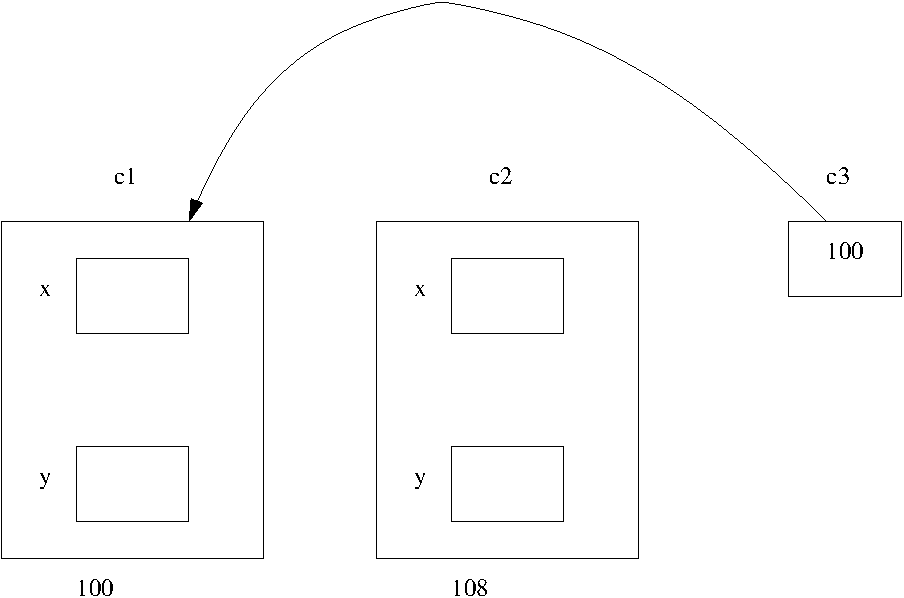
\includegraphics[scale=0.5]{ponteiro_struct}
    \end{center}

\end{frame}

%%%%%%%%%%%%%%%%%%%%%%%%%%%%%%%%%%%%%%%%%%%%%
\begin{frame}[fragile]{Ponteiros e Registros}

    O que será impresso pelo programa abaixo?
    \vspace{-1em}
    \begin{minted}[fontsize=\scriptsize]{c}
        #include <stdio.h>
        struct Coordenada {
            double x;
            double y;
        };
        int main() {
            struct Coordenada c1, c2, *c3;

            c3 = &c1;
            c1.x = -1;
            c1.y = -1.5;

            c2.x = 2.5;
            c2.y = -5;
            *c3 = c2;

            printf("Coordenadas de c1: (%lf,%lf)\n", c1.x, c1.y);
            return 0;
        }
    \end{minted}

\end{frame}

%%%%%%%%%%%%%%%%%%%%%%%%%%%%%%%%%%%%%%%%%%%%%
\begin{frame}[fragile]{Ponteiros e registros}

    Para acessarmos os campos de uma variável \textbf{struct} via um ponteiro,
    podemos utilizar o operador \textbf{*} juntamente com o operador \textbf{.}
    como de costume:

    \begin{minted}{c}
        Coordenada c1, *c3;
        c3 = &c1;
        (*c3).x = 1.5;
        (*c3).y = 1.5;
    \end{minted}

\end{frame}

%%%%%%%%%%%%%%%%%%%%%%%%%%%%%%%%%%%%%%%%%%%%%
\begin{frame}[fragile]{Ponteiros e registros}

    \begin{itemize}
        \item Em C também podemos usar o operador \cod{->}, que
        também é usado para acessar campos de uma estrutura via um
        ponteiro.

        \begin{minted}{c}
            Coordenada c1, *c3;
            c3 = &c1;
            c3->x = 1.5;
            c3->y = 1.5;
        \end{minted}

        \item Resumindo: Para acessar campos de estruturas via
        ponteiros use um dos dois:
        \begin{itemize}
            \item \cod{ponteiroEstrutura->campo}
            \item \cod{(*ponteiroEstrutura).campo}
        \end{itemize}
    \end{itemize}

\end{frame}

%%%%%%%%%%%%%%%%%%%%%%%%%%%%%%%%%%%%%%%%%%%%%
\begin{frame}[fragile]{Ponteiros e registros}

    O que será impresso pelo programa abaixo?
    \vspace{-1em}
    \begin{minted}[fontsize=\scriptsize]{c}
        ...
        int main() {
            struct Coordenada c1, c2, *c3, *c4;
            c3 = &c1;
            c4 = &c2;

            c1.x = -1;
            c1.y = -1.5;
            c2.x = 2.5;
            c2.y = -5;
            (*c3).x = 1.5;
            (*c3).y = 1.5;
            c4->x = -1;
            c4->y = -1;

            printf("Coordenadas de c1: (%lf,%lf)\n",c1.x, c1.y);
            printf("Coordenadas de c2: (%lf,%lf)\n",c2.x, c2.y);
            return 0;
        }
    \end{minted}
\end{frame}

%%%%%%%%%%%%%%%%%%%%%%%%%%%%%%%%%%%%%%%%%%%%%
\begin{frame}[fragile]{Ponteiros e registros}

    Podemos fazer alocação dinâmica de um vetor de registros
    da mesma forma que com tipos simples.

    \begin{minted}{c}
        struct Aluno *vetAlu;
        vetAlu = malloc(10 * sizeof(struct Aluno));
        vetAlu[0].nota = 5.6;
        vetAlu[1].nota = 7.8;
        ...
    \end{minted}

\end{frame}

%%%%%%%%%%%%%%%%%%%%%%%%%%%%%%%%%%%%%%%%%%%%%
\begin{frame}[fragile]{Ponteiros e registros}

    Utilizando as funções criadas anteriormente podemos executar o exemplo:
    \vspace{-1em}
    \begin{minted}[fontsize=\scriptsize]{c}
        struct Aluno leAluno();
        void imprimeAluno(struct Aluno a);
        void listarTurma(struct Aluno turma[], int n);

        int main() {
            struct Aluno *vetAlu;
            int n, i;
            printf("Numero de alunos: ");
            scanf("%d", &n); getchar();

            vetAlu = malloc(n * sizeof(struct Aluno));  /* Alocação dinâmica do vetor de registros */
            for(i = 0; i < n; i++)
                vetAlu[i] = leAluno();
            listarTurma(vetAlu, n);
            free(vetAlu);  /* Liberação de memória alocada */
            return 0;
        }
    \end{minted}

\end{frame}


%%%%%%%%%%%%%%%%%%%%%%%%%%%%%%%%%%%%%%%%%%%%%
%%%%%%%%%%%%%%%%%%%%%%%%%%%%%%%%%%%%%%%%%%%%%
%%%%%%%%%%%%%%%%%%%%%%%%%%%%%%%%%%%%%%%%%%%%%
%%%%%%%%%%%%%%%%%%%%%%%%%%%%%%%%%%%%%%%%%%%%%
%%%%%%%%%%%%%%%%%%%%%%%%%%%%%%%%%%%%%%%%%%%%%
%%%%%%%%%%%%%%%%%%%%%%%%%%%%%%%%%%%%%%%%%%%%%
\section{Exercícios}

%%%%%%%%%%%%%%%%%%%%%%%%%%%%%%%%%%%%%%%%%%%%%
\begin{frame}[fragile]{\exercicio}

    \begin{itemize}
        \item Crie um novo tipo de registro para armazenar coordenadas
        no plano cartesiano.
        \item Crie uma função para imprimir um ponto do tipo criado.
        \item Crie uma função para cada uma destas operações: soma de
        dois pontos, subtração de dois pontos, multiplicação por um
        escalar.
    \end{itemize}

\end{frame}

%%%%%%%%%%%%%%%%%%%%%%%%%%%%%%%%%%%%%%%%%%%%%
%%%%%%%%%%%%%%%%%%%%%%%%%%%%%%%%%%%%%%%%%%%%%
%%%%%%%%%%%%%%%%%%%%%%%%%%%%%%%%%%%%%%%%%%%%%
%%%%%%%%%%%%%%%%%%%%%%%%%%%%%%%%%%%%%%%%%%%%%
%%%%%%%%%%%%%%%%%%%%%%%%%%%%%%%%%%%%%%%%%%%%%
%%%%%%%%%%%%%%%%%%%%%%%%%%%%%%%%%%%%%%%%%%%%%
\section{Informações extras: redefinição de tipos}

%%%%%%%%%%%%%%%%%%%%%%%%%%%%%%%%%%%%%%%%%%%%%
\begin{frame}{Informações extras: redefinido um tipo}

    \begin{itemize}
        \item Às vezes, por questão de organização, gostaríamos de
        criar um tipo próprio nosso, que faz exatamente a mesma coisa
        que um outro tipo já existente.

        \item Por exemplo, em um programa onde manipulamos médias de
        alunos, todas as variáveis que trabalhassem com nota tivessem
        o tipo \textbf{nota}, e não \textbf{double}.
    \end{itemize}

\end{frame}

%%%%%%%%%%%%%%%%%%%%%%%%%%%%%%%%%%%%%%%%%%%%%
\begin{frame}[fragile]{Informações extras: o comando \texttt{typedef}}

    \begin{itemize}
        \item A forma de se fazer isso é utilizando o comando
        \textbf{typedef}, seguindo a sintaxe abaixo:

        \begin{center}
            \begin{minted}{c}
                typedef tipo_já_existente tipo_novo;
            \end{minted}
        \end{center}

        \item Usualmente, fazemos essa declaração fora da função
        \texttt{main()}, embora seja permitido fazer dentro da função
        também. Veja o exemplo:
    \end{itemize}
\end{frame}

\begin{frame}[fragile]{Informações extras: o comando \texttt{typedef}}

    Exemplo: cria tipo \textbf{nota}
    \begin{minted}{c}
        #include <stdio.h>

        typedef double nota;

        int main() {
            nota p1;
            printf("Digite a nota:");
            scanf("%lf", &p1);
            printf("A nota digitada foi: %lf\n", p1);
            return 0;
        }
    \end{minted}
\end{frame}

%%%%%%%%%%%%%%%%%%%%%%%%%%%%%%%%%%%%%%%%%%%%%
\begin{frame}[fragile]{Informações extras: exemplo de uso do \texttt{typedef}}

    \begin{itemize}
        \item O uso mais comum para o comando \textbf{typedef} é para
        a redefinição de tipos registro.
        \item No nosso exemplo de \textbf{struct Aluno}, poderíamos
        redefinir este tipo para algo mais simples como simplesmente
        \textbf{Aluno}:
        \begin{minted}[fontsize=\scriptsize]{c}
            struct Aluno {
                int ra;
                double nota;
            };

            /* redefinimos tipo struct Aluno como Aluno*/
            typedef struct Aluno Aluno;

            int main () {
                Aluno turma[10];
                int i;
                double media;
                ...
            }
        \end{minted}
    \end{itemize}
\end{frame}

%%%%%%%%%%%%%%%%%%%%%%%%%%%%%%%%%%%%%%%%%%%%%
\begin{frame}[fragile]{Informações extras: exemplo de uso do \texttt{typedef}}

    \vspace{-1em}
    \begin{minted}[fontsize=\scriptsize]{c}
        #include <stdio.h>
        struct Aluno {
            int ra;
            double nota;
        };
        typedef struct Aluno Aluno; /* redefine tipo struct Aluno como Aluno */
        int main () {
            Aluno turma[10];
            int i;
            double media = 0.0;
            for (i = 0; i < 10; i++) {
                scanf("%d", &turma[i].ra);
                scanf("%lf", &turma[i].nota);
            }
            /* calcula a media da turma */
            for (i = 0; i < 10; i++)
                media = media + turma[i].nota;
            media = media / 10.0;
            printf("\nA média da turma é: %lf\n", media);
            return 0;
        }
    \end{minted}

\end{frame}

%%%%%%%%%%%%%%%%%%%%%%%%%%%%%%%%%%%%%%%%%%%%%
%%%%%%%%%%%%%%%%%%%%%%%%%%%%%%%%%%%%%%%%%%%%%
%%%%%%%%%%%%%%%%%%%%%%%%%%%%%%%%%%%%%%%%%%%%%
%%%%%%%%%%%%%%%%%%%%%%%%%%%%%%%%%%%%%%%%%%%%%
%%%%%%%%%%%%%%%%%%%%%%%%%%%%%%%%%%%%%%%%%%%%%
%%%%%%%%%%%%%%%%%%%%%%%%%%%%%%%%%%%%%%%%%%%%%
\section{Informações extras: tipos enumerados}

%%%%%%%%%%%%%%%%%%%%%%%%%%%%%%%%%%%%%%%%%%%%%
\begin{frame}[fragile]{Tipos enumerados}

    \begin{itemize}
        \item Para criar uma variável para armazenar um determinado mês
        de um ano (de janeiro a dezembro), uma das soluções possíveis
        é criar um inteiro e armazenar um número associado àquele mês.
        Assim, janeiro seria o mês número 1, fevereiro o mês número 2,
        e assim sucessivamente.

        \item Mas, o código seria mais claro se pudéssemos escrever algo como:

        \begin{center}
            \alert{\cod{mes = janeiro;}}
        \end{center}
    \end{itemize}

\end{frame}

%%%%%%%%%%%%%%%%%%%%%%%%%%%%%%%%%%%%%%%%%%%%%
\begin{frame}[fragile]{Tipos enumerados: (\texttt{enum})}

    \begin{itemize}
        \item O comando \texttt{enum} cria um tipo enumerado:
        podemos usar nomes/identificadores para um conjunto finito
        de valores inteiros.

        \item Sua sintaxe é:

        \begin{block}{}
            \begin{minted}[linenos=false,frame=none]{c}
                enum nomeDoTipo {identificador1, identificador2, ...
                  identificadorn};
            \end{minted}
        \end{block}

        \item Exemplo:
        \begin{minted}{c}
            /* criamos um novo tipo chamado "enum meses" */
            enum meses {jan, fev, mar, abr, mai, jun,
                        jul, ago, set, out, nov, dez};

        \end{minted}
    \end{itemize}

\end{frame}

%%%%%%%%%%%%%%%%%%%%%%%%%%%%%%%%%%%%%%%%%%%%%
\begin{frame}[fragile]{Tipos enumerados: \texttt{enum}}

    \begin{itemize}
        \item O compilador associa o número 0 para o primeiro
        identificador, 1 para o segundo, etc.
        \item Variáveis do novo tipo criado são na realidade variáveis
        inteiras.
        \item Tipos enumerados são usados para deixar o código mais
        legível.
    \end{itemize}

\end{frame}

%%%%%%%%%%%%%%%%%%%%%%%%%%%%%%%%%%%%%%%%%%%%%
\begin{frame}[fragile]{Tipos enumerados: \texttt{enum}}

    \begin{minted}[fontsize=\scriptsize]{c}
        #include<stdio.h>
        /* aqui criamos um novo tipo enumerado que pode ser usado por qualquer
        função */
        enum meses {jan, fev, mar, abr, mai, jun, jul, ago, set, out, nov, dec};

        int main() {
            enum meses a, b; /* cria 2 variáveis do tipo "enum meses" */

            a = jan;
            b = jun;

            if (a != b) {
                /* será impresso "0 é um mes diferente de 5" */
                printf("%d é um mes diferente de %d\n", a, b);
            }
            return 0;
        }
    \end{minted}

\end{frame}

%%%%%%%%%%%%%%%%%%%%%%%%%%%%%%%%%%%%%%%%%%%%%
\begin{frame}[fragile]{Usando um tipo enumerado}

    \begin{itemize}
        \item Note que o primeiro identificador recebeu o valor zero,
        e demais identificadores receberam valores em sequência.
        \item Podemos alterar o valor inicial dos identificadores.
    \end{itemize}

    \begin{minted}[fontsize=\scriptsize]{c}
        #include<stdio.h>
        enum meses {jan = 1, fev, mar, abr, mai, jun, jul, ago, set, out, nov, dec};

        int main() {
            enum meses a, b; /* cria 2 variáveis do tipo "enum meses" */

            a = jan;
            b = jun;

            if (a != b) {
                /* será impresso "1 é um mes diferente de 6" */
                printf("%d é um mes diferente de %d", a, b);
            }
            return 0;
        }
    \end{minted}

\end{frame}

%%%%%%%%%%%%%%%%%%%%%%%%%%%%%%%%%%%%%%%%%%%%%
\begin{frame}{Tipos enumerados: resumindo}

    \begin{itemize}
        \item Um tipo enumerado pode ser criado para deixar o código
        mais legível.
        \item Variáveis de um tipo enumerado criado, são na realidade
        variáveis inteiras, mas temos a versatilidade de atribuir os
        identificadores do tipo enumerado para tais variáveis.
    \end{itemize}

\end{frame}

\end{document}
